\documentclass[aspectratio=169]{beamer}

% Custom theme and packages
\usepackage{beamertheme-custom}
% Custom symbols and commands
\usepackage{symbols-custom}

\graphicspath{{../figures/}}

\title{Everybody stroops}
\author{Joachim Vandekerckhove}
\date{Spring 2025}

\titlegraphic{\hfill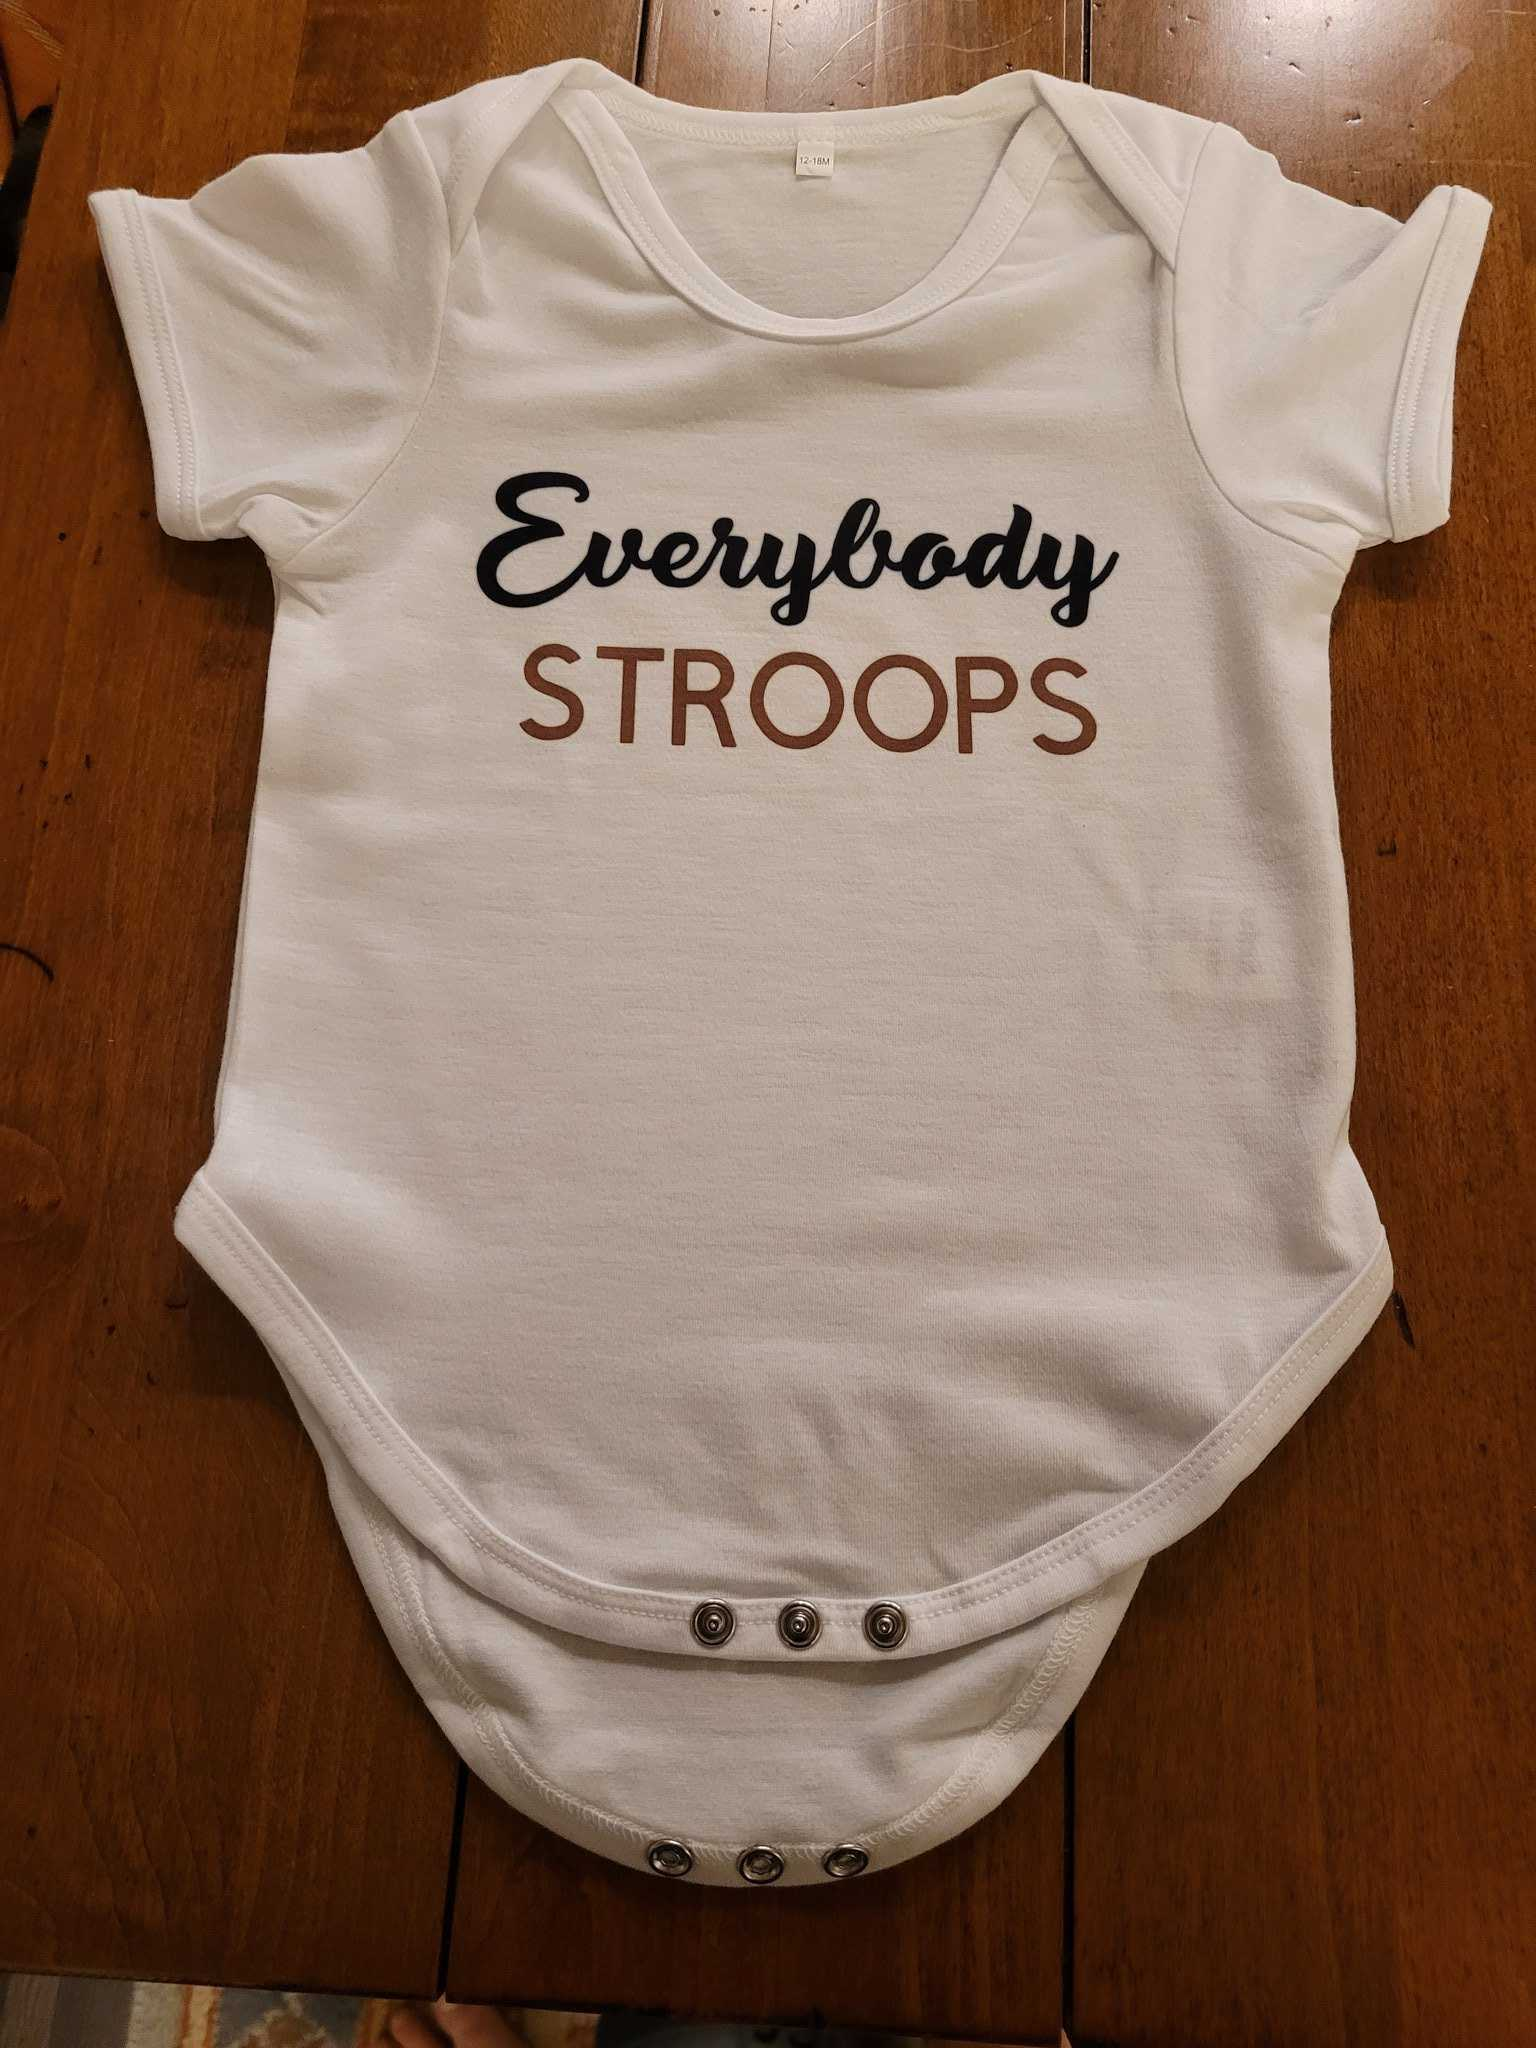
\includegraphics[scale=.045]{everybody-stroops.jpg}}

% Font
\usefonttheme[onlymath]{serif}


\begin{document}

\maketitle

\begin{frame}[fragile]{Speeded choice response time}

\ex{Speeded response times (aka reaction times)}
These result from easy tasks where the participant is instructed to respond as quickly as possible.  They happen on short time scales -- \emph{less than a second on average}.  You might call them `split-second' decisions.  Real life examples are tasks such as deciding when to brake while driving, or whether to duck or jump if an object flies your way.
\xe\pause

\ex{Choice response times}
These result from tasks in which the participant is specifically instructed to choose between several alternatives.  They not only have to press a button but additionally have to \emph{choose which button} to press.  There may be two alternatives (two-choice response times) or more than two (multialternative response times).
\xe

\end{frame}



\begin{frame}[fragile]{Visualizing CRT data}

\emph{Quantiles} can be used to summarize nonstandard distributions\\[2ex]\pause

\begin{figure}[htp]
\centering
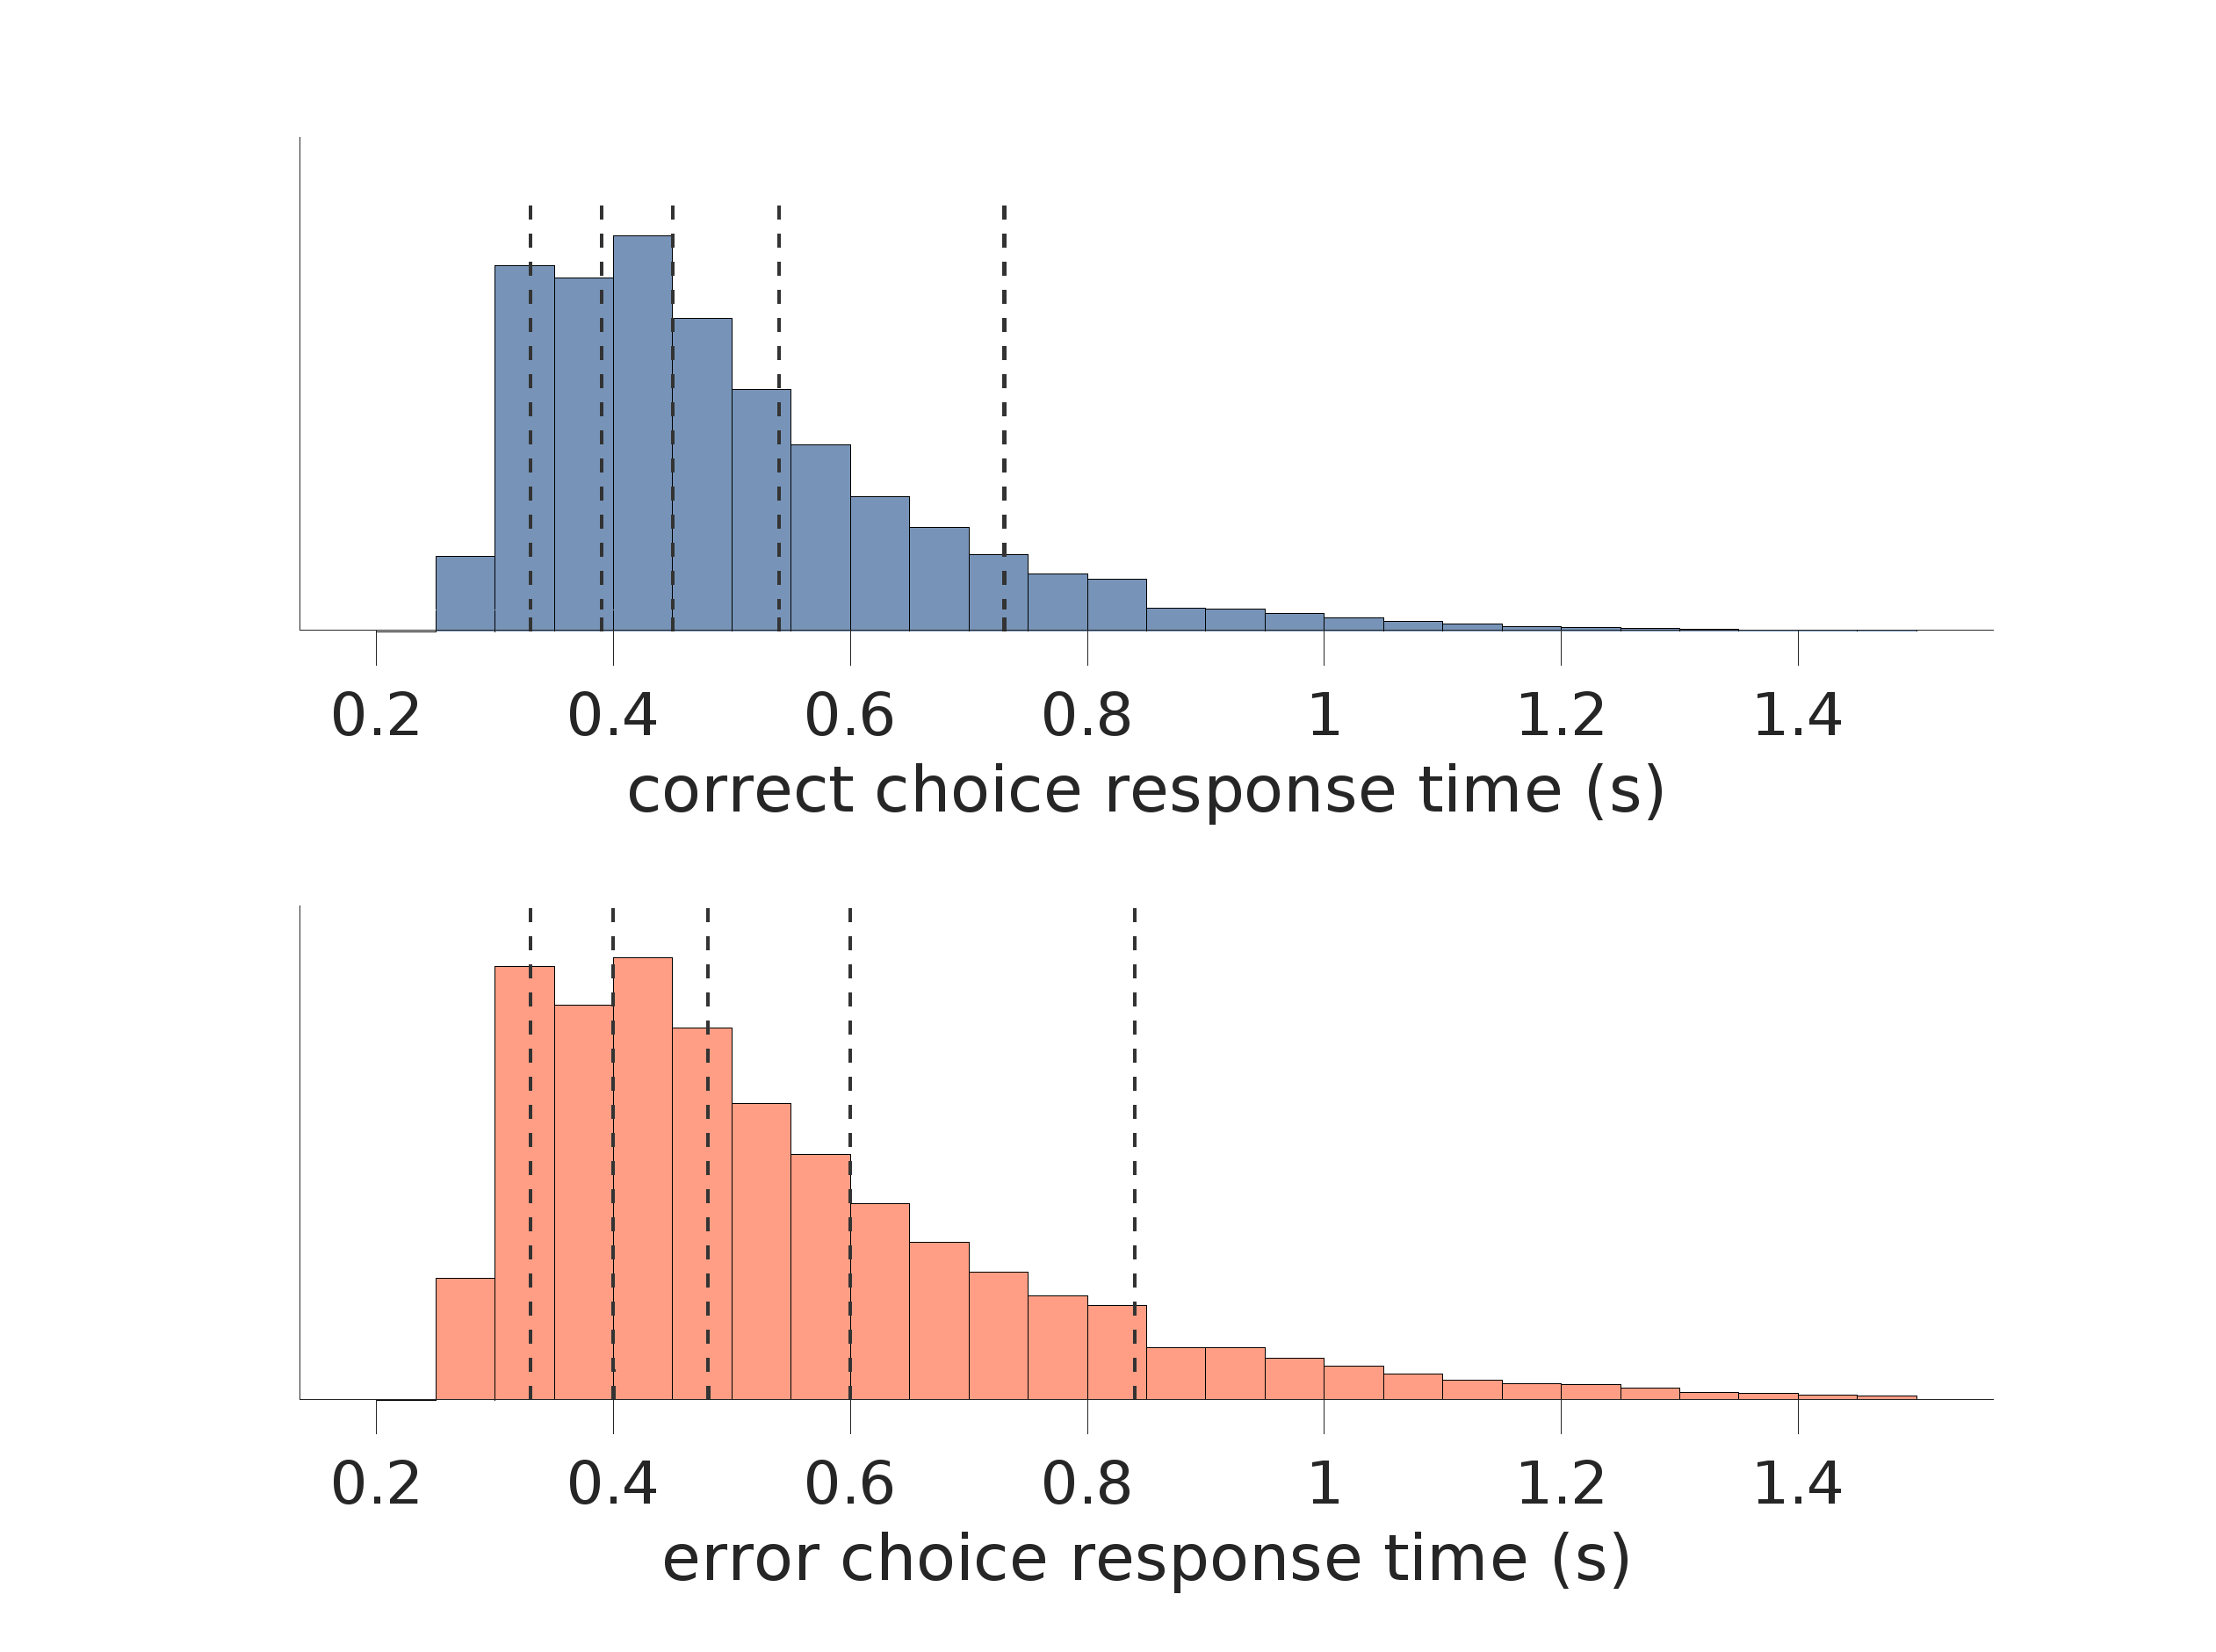
\includegraphics[scale=0.18]{rtdist6}
\end{figure}

\end{frame}


\begin{frame}[fragile]{Direct comparison of quantiles}
\begin{figure}[htp]
\centering
\includegraphics<1>[width=\textwidth]{deltasmall0.eps}%
\includegraphics<2>[width=\textwidth]{deltasmall1.eps}%
\includegraphics<3>[width=\textwidth]{deltasmall2.eps}
\end{figure}
\only<1->{$$\Delta_n = P_n(t_2) - P_n(t_1)$$}

\end{frame}



\begin{frame}[fragile]{Delta plots}
\begin{minipage}{.135\textwidth}\centering
\begin{tabular}{cc}
$\Delta_{10} = 0.05$\\
$\Delta_{30} = 0.08$\\
$\Delta_{50} = 0.11$\\
$\Delta_{70} = 0.13$\\
$\Delta_{90} = 0.17$\\
\end{tabular}
\end{minipage}
\begin{minipage}{.85\textwidth}
\begin{figure}[htp]
\centering
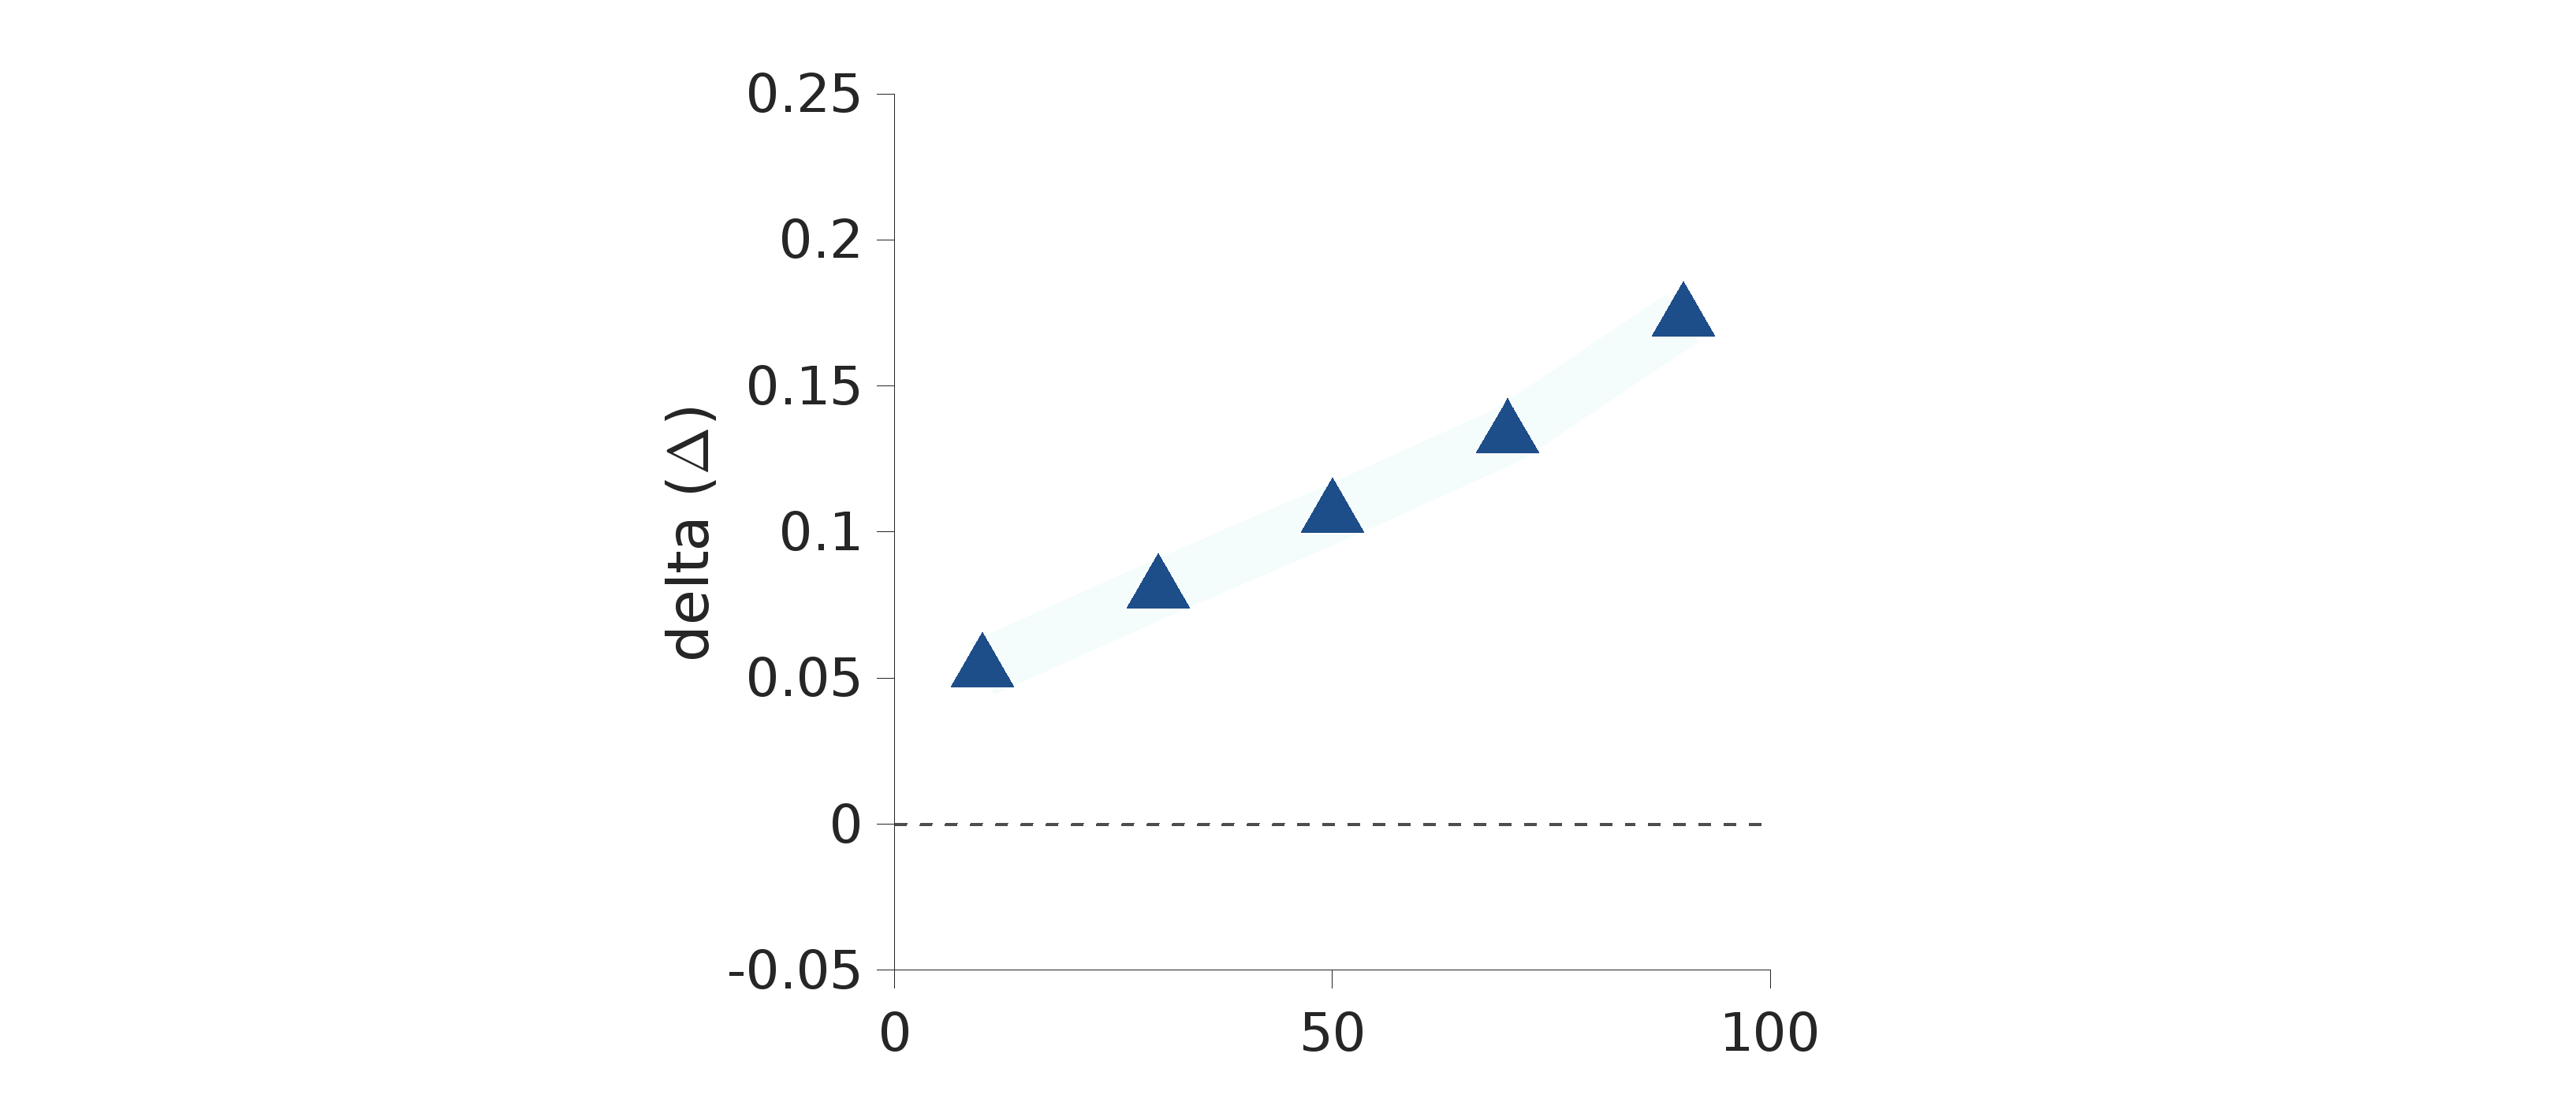
\includegraphics[scale=0.2,bb=00 0 1100 655,clip]{deltasmall3.eps}
\end{figure}
\end{minipage}\vspace{2ex}

Delta plots can quickly reveal patterns of effects due to experimental manipulations 
\end{frame}


\definecolor{verylightgray}{rgb}{.9,.9,.9}



\begin{frame}[fragile]{Diffusion models for two-choice response times}\centering
\begin{tabular}{cll}
\rowcolor{black}
           & {\it\color{white}parameter} &  {\it\color{white}interpretation} \\
\rowcolor{verylightgray}
$\delta$   &  drift rate              &  dominance ($\eta$, $d'$) \\
\rowcolor{lightgray}
$\alpha$   &  boundary separation     &  caution \\
\rowcolor{verylightgray}
$\tau$     &  nondecision time        &  time for encoding and responding \\
\rowcolor{lightgray}
$\beta$    &  initial bias            &  a priori response bias \\
\end{tabular}

\begin{figure}[htp]
\centering
{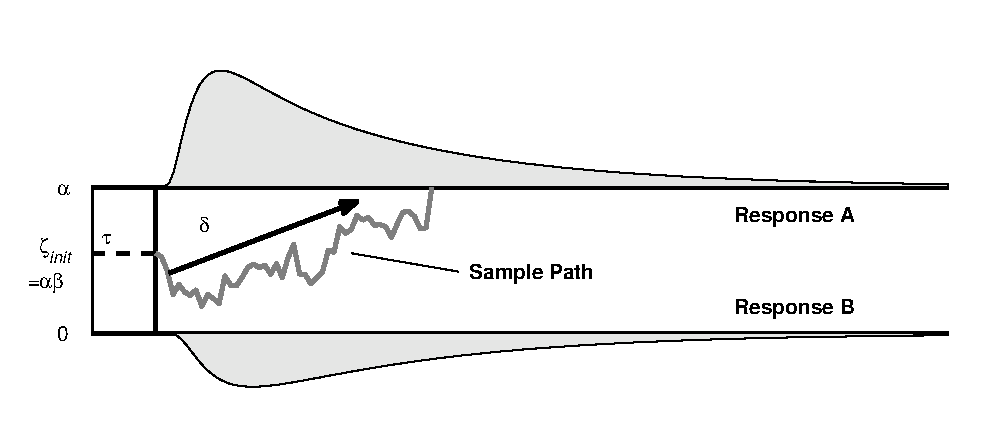
\includegraphics[scale=0.6]{rdmpmeth.eps}}
\end{figure}
\end{frame}



\begin{frame}[fragile]{Diffusion model parameters in delta plots}

Diffusion model parameter effects become tell-tale patterns in delta plots\\[4ex]

 \centering
\begin{tabular}{cll}
\rowcolor{black}
           & {\it\color{white}parameter} &  {\it\color{white}interpretation} \\
\rowcolor{verylightgray}
$\delta$   &  drift rate              &  dominance ($\eta$, $d'$) \\
\rowcolor{lightgray}
$\alpha$   &  boundary separation     &  caution \\
\rowcolor{verylightgray}
$\tau$     &  nondecision time        &  time for encoding and responding
\end{tabular}

\begin{figure}[htp]
\centering
\vspace{-2ex}
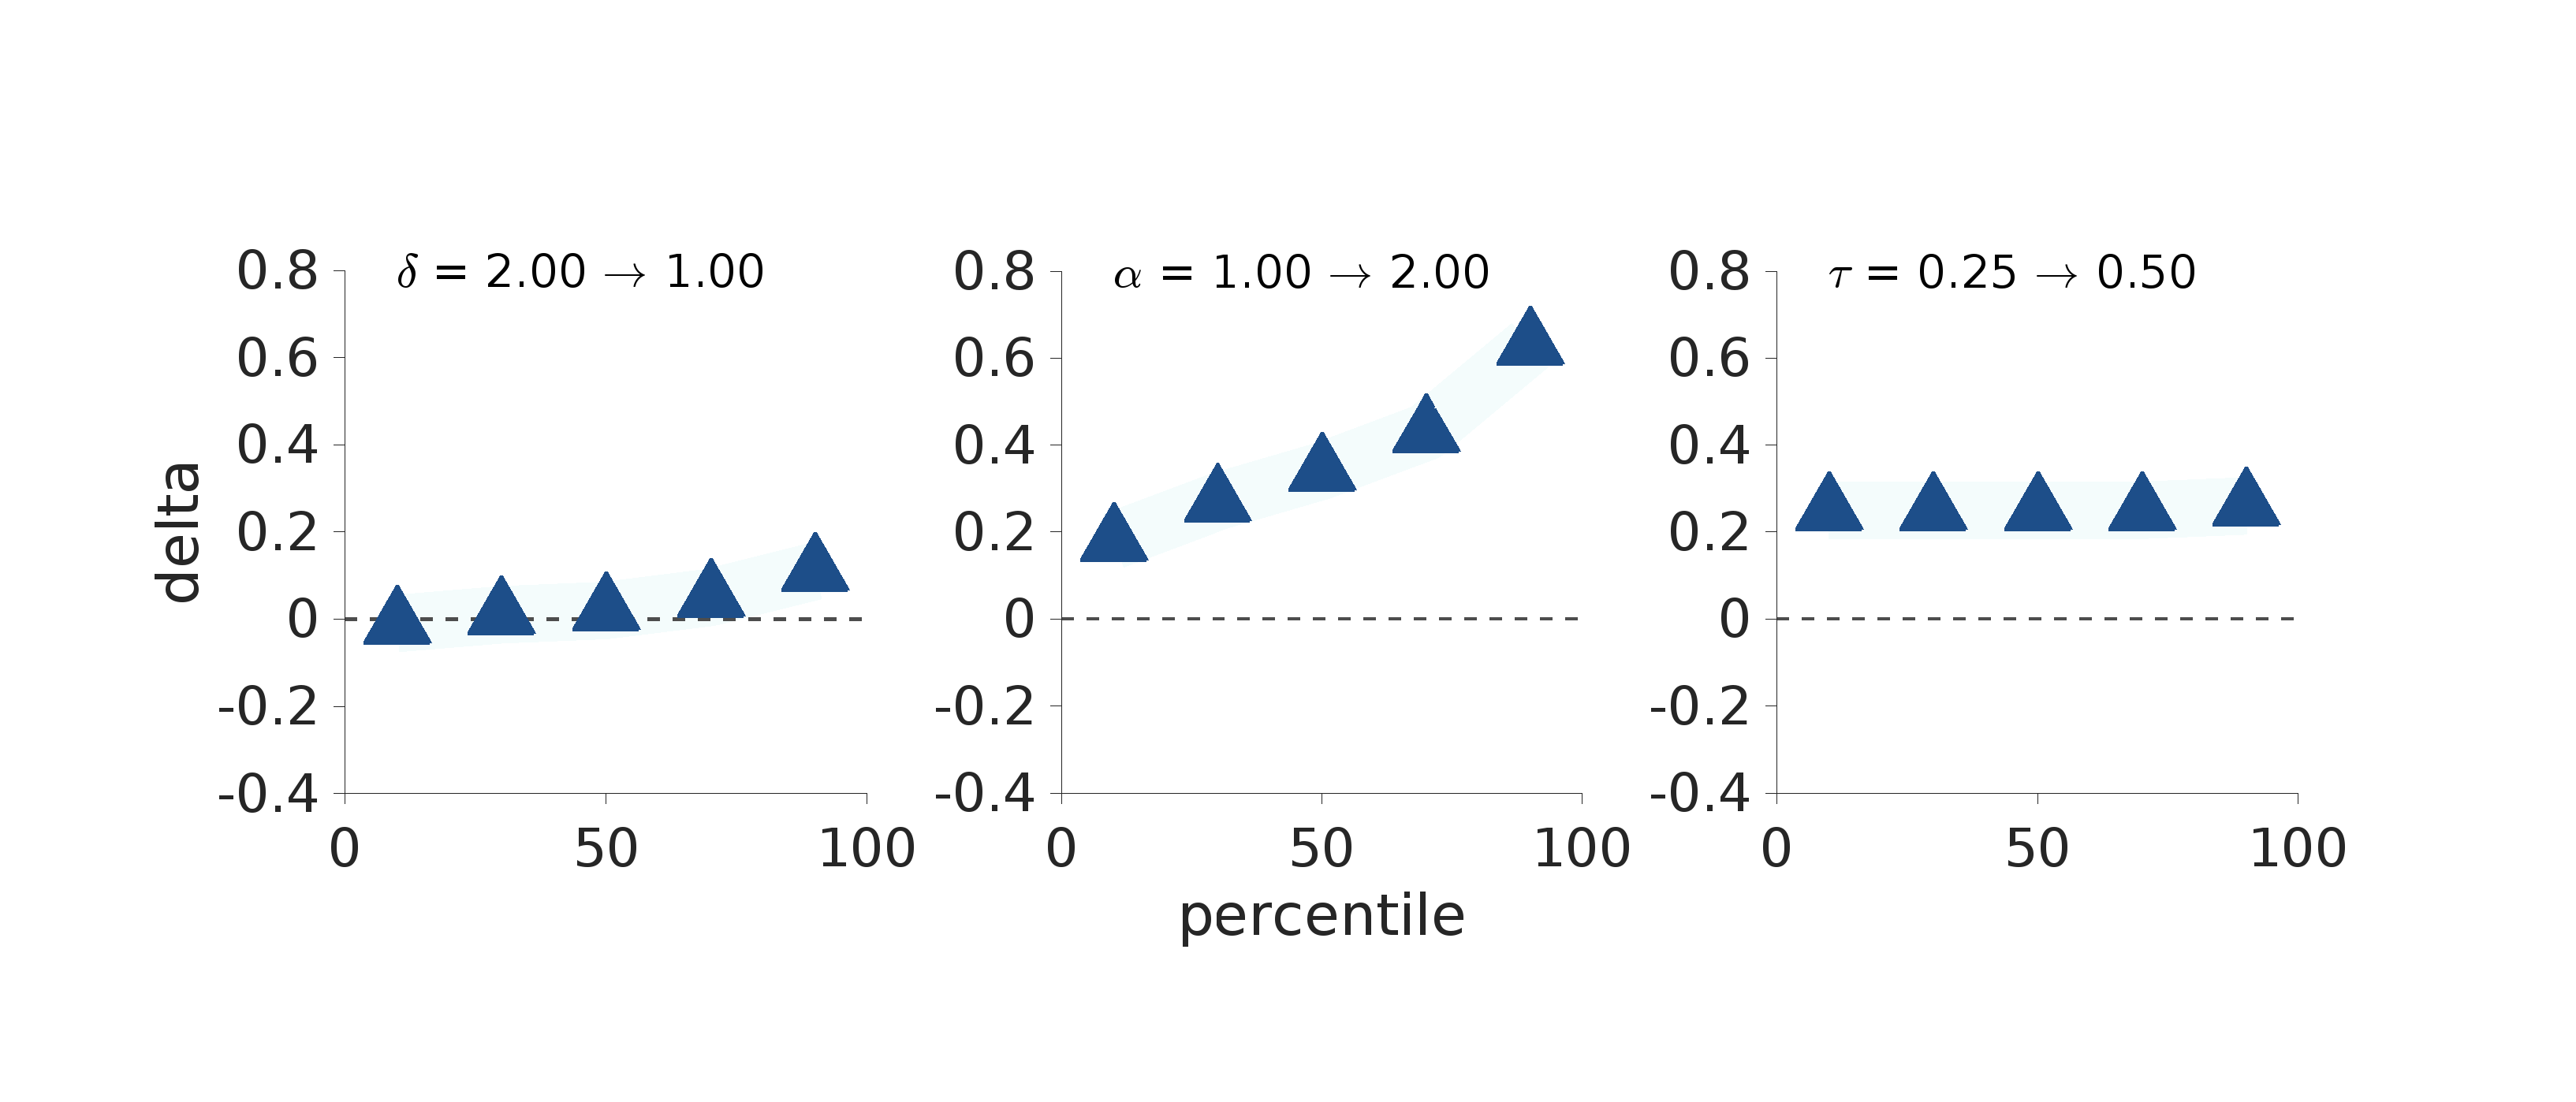
\includegraphics[scale=0.18,bb= 0 0 1552 600,clip]{deltadiff.eps}
\end{figure}

\end{frame}



\begin{frame}{EZ diffusion}
  \begin{itemize}
    \item The \emph{Simple DDM} is a three-parameter model that accounts for choice and RT data using a Wiener likelihood function.\pause
    \item The likelihood of the DDM is quite complicated so maximum likelihood estimation can be slow.\pause
    \item Sampling from the DDM is not so difficult but a little time consuming.
  \end{itemize}
\end{frame}




\begin{frame}{EZ diffusion}
  \begin{itemize}
    \item The \emph{EZ diffusion model} is a simplified method that allows us to compute estimated parameters directly from observed summary statistics.\\\pause
    \item A lot like signal detection theory, but with response times).\\\pause
    \item[]\vspace{2ex}
    \begin{tabular}{l@{$\qquad\leftrightarrow\qquad$}l}
    
    \begin{tabular}{ll}
    \hline
      Summary statistics &  \\
      \hline
      Accuracy rate & $\ObservedAccuracyRate$ \\
      Mean RT & $\ObservedMean$ \\
      Variance RT & $\ObservedVariance$\\
    \hline
    \end{tabular}\pause
&
    \begin{tabular}{ll}
    \hline
       Parameters \\
      \hline
      Drift rate & $\EstDrift$ \\
      Boundary separation & $\EstBound$ \\
      Nondecision time & $\EstNondecision$\\
    \hline
    \end{tabular}
    \end{tabular}
    \vspace{4ex}\pause
    \item EZ diffusion involves two sets of equations, the \emph{forward} equations give the summary statistics in terms of parameters, and the \emph{inverse} equations give the parameters in terms of summary statistics. 
  \end{itemize}
\end{frame}


\begin{frame}{EZ diffusion -- forward}
\emph{Forward} EZ equations:
\begin{eqnarray}
    \PredAccuracyRate &=& \frac{1}{y + 1}
    \label{eq:ez:forward:Ma}
    \\
    \PredMean         &=&
        \nondt + \left(\frac{\bound}{2 \drift}\right)
        \left(\frac{1 - {y}}{1 + {y}}\right),
    \label{eq:ez:forward:Mt}
    \\
    \PredVariance     &=&  
        \left(\frac{\bound}{2\drift^3}\right)
        \left\{\frac{1-2\bound\drift{y} - {y}^2}{\left({y} + 1\right)^2}\right\}
    \label{eq:ez:forward:Vt}
\end{eqnarray}
with $y = \exp\left(-\bound \drift\right)$.
\end{frame}




\begin{frame}{EZ diffusion -- inverse}
\emph{Inverse} EZ equations:
\begin{eqnarray}
    \EstDrift &=& \sign{\ObservedAccuracyRate - \frac{1}{2}} \sqrt[\Huge{4}]{\frac{\LogitAccuracy\left(\ObservedAccuracyRate^2 \LogitAccuracy - \ObservedAccuracyRate   \LogitAccuracy + \ObservedAccuracyRate - \frac{1}{2}\right)}{\ObservedVariance}}\\
    \EstBound &=& \frac{\LogitAccuracy}{\EstDrift}\\
    \EstNondecision &=& \ObservedMean - \left(\frac{\EstBound}{2\EstDrift}\right) \left[\frac{1-\text{exp}\left({-\EstDrift\EstBound}\right)}{1+\text{exp}\left({-\EstDrift\EstBound}\right)}\right].
\end{eqnarray}
with $\LogitAccuracy = \log\left(\frac{\ObservedAccuracyRate}{1-\ObservedAccuracyRate}\right)$.
\end{frame}





\begin{frame}{EZ diffusion}
This is extremely useful, because now we can calculate these interesting parameters without having to use complicated numerical algorithms.\pause

But something is missing here!  How would we go about putting these equations in a PyMC model.\pause

Note there are no distributions, there is no likelihood function here.\pause

There is a solution that requires a bit of statistical manipulation,
\end{frame}


\begin{frame}{EZ diffusion -- sampling distributions}
If $\TrialsTotal$ observations are drawn from a diffusion model whose accuracy rate is $\PredAccuracyRate$, then the sampling distribution of the observed number of correct trials $\ObservedAccuracyTotal = N \times \ObservedAccuracyRate$ is:
\begin{equation}
    \ObservedAccuracyTotal \sim \text{Binomial}\left(\PredAccuracyRate,\TrialsTotal\right).\label{eq:accuracy}
\end{equation}\pause
If $\TrialsTotal$ observations are drawn from a sample whose mean and variance of the RTs are $\PredMean$ and $\PredVariance$, then the sampling distribution of the observed mean RT $\ObservedMean$ is:
\begin{equation}
    \ObservedMean \sim \text{Normal}\left(\PredMean,\frac\PredVariance\TrialsTotal\right).\label{eq:mean}
\end{equation}\pause
And the sampling distribution of the variance of the RTs follows this probability law:
\begin{equation}
    \ObservedVariance \sim \text{Gamma}\left(\frac{\TrialsTotal-1}{2}, \frac{2\PredVariance}{\TrialsTotal-1}\right).
    \label{eq:var}
\end{equation}
\end{frame}


\begin{frame}{EZ diffusion -- a likelihood}
These sampling statements form a likelihood!\pause

Define $Y_{pc} = \left(\ObservedAccuracyTotal_{pc}, \ObservedMean_{pc}, \ObservedVariance_{pc}\right)$\pause
$$Y_{pc} \sim EZ\left(\drift_{pc},\bound_{pc},\nondt_{pc}\right)$$\pause
Now we can once again apply our parameter decomposition techniques to cognitive model distributions:
$$ \delta_{pc} = \mu + \beta \text{Condition}_c + \varepsilon_p $$\pause
(Except now the computation takes seconds instead of days.)
\end{frame}



\begin{frame}[fragile]{Stroop Stroop}
\pause
\begin{center}
\huge
\begin{tabular}{c@{\hspace{5em}}c}
{\color{blue} \bfseries green}  & {\color{green} \bfseries green}  \\
{\color{green}\bfseries red}    & {\color{red}   \bfseries red}    \\
{\color{black}\bfseries orange} & {\color{orange}\bfseries orange} \\
{\color{red}  \bfseries blue}   & {\color{blue}  \bfseries blue}  
\end{tabular}
\end{center}
\end{frame}



\begin{frame}[fragile]{Stroop Stroop}
\begin{center}
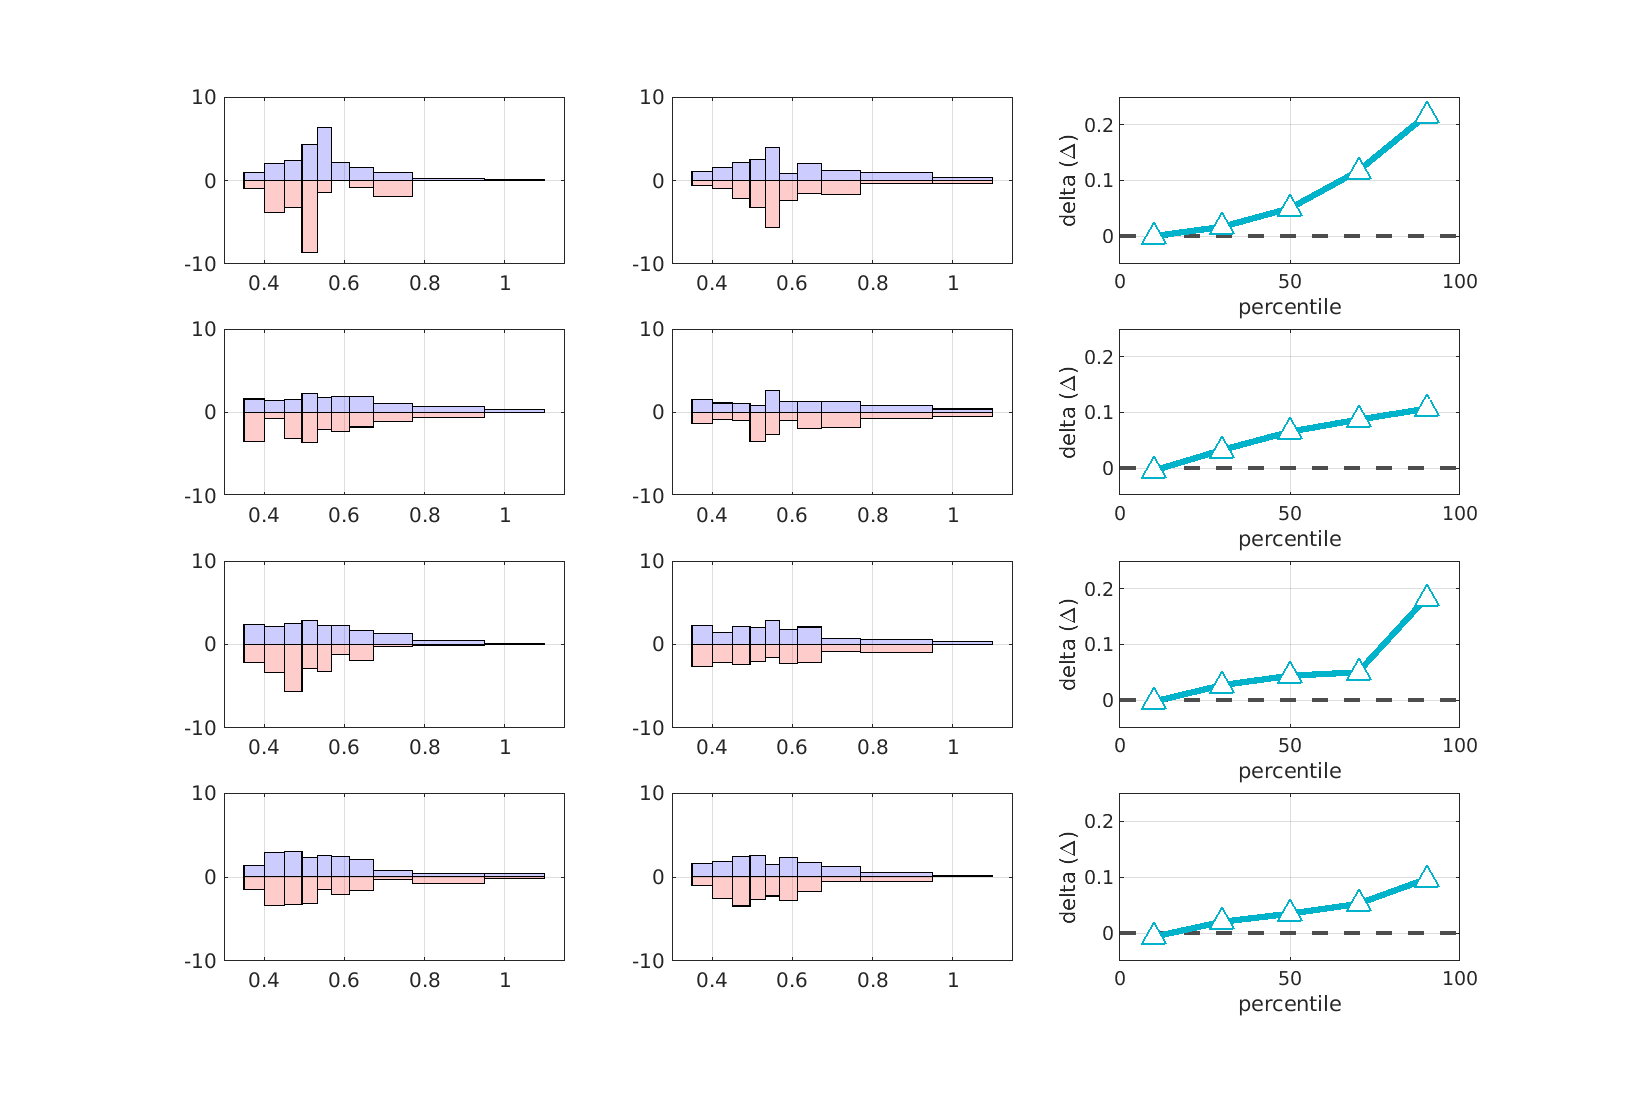
\includegraphics[scale=.5,trim=80 10 80 30]{rts}
\end{center}
\end{frame}




\begin{frame}[fragile]{Stroop Stroop --- Ability~$\delta$}
\begin{table}[h]
	\centering\scriptsize
	\label{tab:mCMCSummary}
	{
		\begin{tabular}{lrrrrrrrr}
			\toprule
			\multicolumn{1}{c}{} & \multicolumn{3}{c}{Posterior} & \multicolumn{2}{c}{95\% Cr.\ Int.} & \multicolumn{2}{c}{Rhat} & \multicolumn{1}{c}{} \\
			\cline{2-4}\cline{5-6}\cline{7-8}
			Parameter & Mean & Median & SD & Lower & Upper & Point & Upper & ESS  \\
			\cmidrule[0.4pt]{1-9}
			delta[1] & $1.540$ & $1.542$ & $0.106$ & $1.332$ & $1.745$ & $1.005$ & $1.012$ & $1419$  \\
			delta[2] & $0.991$ & $0.993$ & $0.132$ & $0.725$ & $1.245$ & $1.002$ & $1.008$ & $2997$  \\
			delta[3] & $1.407$ & $1.407$ & $0.106$ & $1.207$ & $1.619$ & $1.001$ & $1.005$ & $1619$  \\
			delta[4] & $1.004$ & $1.005$ & $0.097$ & $0.809$ & $1.196$ & $1.002$ & $1.009$ & $2197$  \\
			delta[5] & $1.508$ & $1.510$ & $0.129$ & $1.254$ & $1.752$ & $1.000$ & $1.002$ & $1927$  \\
			delta[6] & $1.282$ & $1.287$ & $0.113$ & $1.048$ & $1.499$ & $1.005$ & $1.010$ & $2008$  \\
			delta[7] & $1.452$ & $1.453$ & $0.131$ & $1.188$ & $1.700$ & $1.001$ & $1.006$ & $2061$  \\
			delta[8] & $1.228$ & $1.228$ & $0.109$ & $1.011$ & $1.437$ & $1.002$ & $1.004$ & $1805$  \\
			\bottomrule
			% \addlinespace[1ex]
			% \multicolumn{9}{p{0.5\linewidth}}{\textit{Note.} Output based on 6000 MCMC draws.} \\
			% \multicolumn{9}{p{0.5\linewidth}}{\textit{Note.} The multivariate potential scale reduction factor is estimated at 1.018.} \\
		\end{tabular}
	}
\end{table}

\centering

{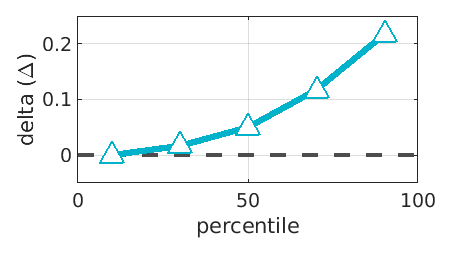
\includegraphics[scale=.35]{d1.eps}}
{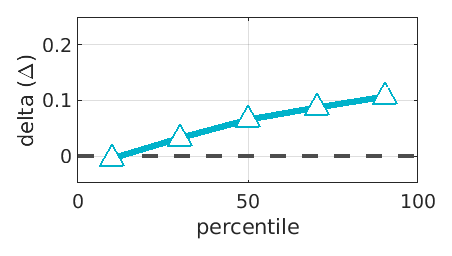
\includegraphics[scale=.35]{d2.eps}}
{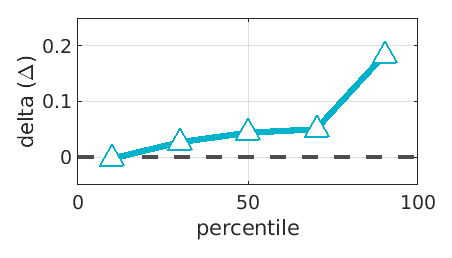
\includegraphics[scale=.35]{d3.eps}}
{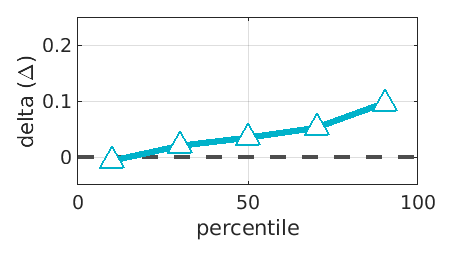
\includegraphics[scale=.35]{d4.eps}}

\end{frame}


\begin{frame}[fragile]{Stroop Stroop --- Nondecision Time~$\tau$}
\begin{table}[h]
	\centering\scriptsize
	\label{tab:mCMCSummary}
	{
		\begin{tabular}{lrrrrrrrr}
			\toprule
			\multicolumn{1}{c}{} & \multicolumn{3}{c}{Posterior} & \multicolumn{2}{c}{95\% Cr.\ Int.} & \multicolumn{2}{c}{Rhat} & \multicolumn{1}{c}{} \\
			\cline{2-4}\cline{5-6}\cline{7-8}
			Parameter & Mean & Median & SD & Lower & Upper & Point & Upper & ESS  \\
			\cmidrule[0.4pt]{1-9}
			tau[1] & $0.178$ & $0.179$ & $0.029$ & $0.117$ & $0.232$ & $1.004$ & $1.015$ & $1917$  \\
			tau[2] & $0.389$ & $0.390$ & $0.020$ & $0.347$ & $0.426$ & $1.002$ & $1.008$ & $1888$  \\
			tau[3] & $0.321$ & $0.323$ & $0.028$ & $0.264$ & $0.372$ & $1.003$ & $1.006$ & $1966$  \\
			tau[4] & $0.313$ & $0.315$ & $0.035$ & $0.241$ & $0.378$ & $1.005$ & $1.018$ & $2108$  \\
			tau[5] & $0.316$ & $0.317$ & $0.020$ & $0.274$ & $0.352$ & $1.004$ & $1.015$ & $1968$  \\
			tau[6] & $0.297$ & $0.298$ & $0.026$ & $0.244$ & $0.345$ & $1.001$ & $1.002$ & $1990$  \\
			tau[7] & $0.344$ & $0.345$ & $0.019$ & $0.306$ & $0.378$ & $1.003$ & $1.011$ & $2048$  \\
			tau[8] & $0.275$ & $0.276$ & $0.028$ & $0.218$ & $0.326$ & $1.001$ & $1.002$ & $2061$  \\
			\bottomrule
			% \addlinespace[1ex]
			% \multicolumn{9}{p{0.5\linewidth}}{\textit{Note.} Output based on 6000 MCMC draws.} \\
			% \multicolumn{9}{p{0.5\linewidth}}{\textit{Note.} The multivariate potential scale reduction factor is estimated at 1.018.} \\
		\end{tabular}
	}
\end{table}
\end{frame}

\begin{frame}[fragile]{Stroop Stroop --- Caution~$\alpha$}
\begin{table}[h]
	\centering\scriptsize
	\label{tab:mCMCSummary}
	{
		\begin{tabular}{lrrrrrrrr}
			\toprule
			\multicolumn{1}{c}{} & \multicolumn{3}{c}{Posterior} & \multicolumn{2}{c}{95\% Cr.\ Int.} & \multicolumn{2}{c}{Rhat} & \multicolumn{1}{c}{} \\
			\cline{2-4}\cline{5-6}\cline{7-8}
			Parameter & Mean & Median & SD & Lower & Upper & Point & Upper & ESS  \\
			\cmidrule[0.4pt]{1-9}
			alpha[1] & $1.513$ & $1.510$ & $0.064$ & $1.396$ & $1.646$ & $1.010$ & $1.032$ & $997$  \\
			alpha[2] & $1.039$ & $1.037$ & $0.033$ & $0.980$ & $1.107$ & $1.002$ & $1.008$ & $1445$  \\
			alpha[3] & $1.408$ & $1.404$ & $0.052$ & $1.313$ & $1.517$ & $1.002$ & $1.005$ & $1181$  \\
			alpha[4] & $1.461$ & $1.458$ & $0.047$ & $1.377$ & $1.562$ & $1.007$ & $1.023$ & $1313$  \\
			alpha[5] & $1.145$ & $1.144$ & $0.040$ & $1.072$ & $1.230$ & $1.002$ & $1.007$ & $1231$  \\
			alpha[6] & $1.301$ & $1.299$ & $0.044$ & $1.221$ & $1.393$ & $1.002$ & $1.008$ & $1155$  \\
			alpha[7] & $1.080$ & $1.078$ & $0.036$ & $1.015$ & $1.156$ & $1.003$ & $1.009$ & $1323$  \\
			alpha[8] & $1.333$ & $1.331$ & $0.045$ & $1.251$ & $1.423$ & $1.001$ & $1.003$ & $1281$  \\
			\bottomrule
		\end{tabular}
	}
\end{table}
\nocite{zhang2014time}

\end{frame}

\begin{frame}{Steps of a diffusion modeling study}

Suppose you are asked to determine if some experimental manipulation $Q_c$ has an effect on information processing speed or nondecisional components, and if the effect is different between participant groups $A$ and $B$.

\begin{enumerate}
\item Make some delta plots of the data, and visually inspect the patterns
\item Construct and run a model that has parameters for the relevant effect sizes
$$\delta_{pc} = \mu + \beta_1 Q_c + \beta_2 B_p + \beta_3 Q_c B_p + \varepsilon_p $$
\item Thoroughly evaluate the convergence of the model with tables and figures
\item Characterize the posterior distributions
\end{enumerate}

\end{frame}


\maketitle

\end{document}
